\chapter{Testing}

This section covers property testing using QuickCheck, system testing using a 
built-in test suite and MySQL WorkBench for SQL query testing. EFA's 
implementation uses dependent types which express application-specific program 
invariants that are beyond the scope of existing type systems. The tests that 
are implemented make two assumptions, the first being any element reused from 
the Ampersand system is already correct, and the second being that if the 
properties of a function are correctly implemented, when used in combination 
with assumption one that the outcome is correct.

\section{Property Testing Using QuickCheck}
Not all functions can be tested using QuickCheck due to their complexity (e.g. 
eca2SQL). All of EFA's modules rely on a few base modules, and testing the 
properties of the functions implemented in the base modules, by extension, 
tests all functions that rely on these core modules. These tests can be checked 
using stack and running \verb|``quickCheck <function>''|. The data types are 
presumed correct as they produce the correct results and are accepted by the 
Ampersand system. Furthermore, proof of EFA's TypedSQL was provided in software 
implementation section \ref{subsec:modhierarchy}

\subsubsection*{Singletons.singKindWitness1}
For every pair of types and their type representation, an isomorphism exists,
where an isomorphism is a morphism $f:\ a \rightarrow b$ and there exists a
morphism $g: b \rightarrow a$ with $fg$ = $1_b$ and $gf$ = $1_a$. The default
implementation uses \lstinline{unsafeCoerce} and will only work if everything
is correctly defined.
         

\subsubsection*{Singletons.sing2val and Singletons.val2sing}
sing2val takes a singleton for some type and converts it to the value
from which it was promoted (e.g. \lstinline{'True} becomes \lstinline{True}).
val2sing does the opposite, except that it must return its output 
existentially quantified. These functions should be witnesses to the isomorphism
between singletons and their unlifted types, i.e it should be the case
that \lstinline{sing2val . val2sing = id} and \lstinline{val2sing . sing2val = id}. 


\subsubsection*{Singletons.$\boldsymbol{(\%==)}$} 
This function implements equality between types by induction on their singletons.
This function (when viewed as a binary relation) should be an equivalence, 
so therefore symmetry, transitive, and reflexive. 

\begin{description}[labelindent=1cm]
\item[Transitivity] $\forall\ a,\ b,\ c \in  X$ : ($aRb \wedge bRc$)$ \Rightarrow\ aRc$
\item[Reflexivity] $\forall a \in\ X $($aRa$)  
\item[Symmetry] $\forall a, b, \in X$ ($aRb \Rightarrow bRa$) 
\end{description}

\subsubsection*{Utils.foldrProd}
This function, and similarly \lstinline{Utils}.\lstinline{foldlProd} implement
the natural fold over the \lstinline{Prod} type, in the same way that 
the function \lstinline{foldr} acts upon lists. This function
must satisfy the property that it behaves the same as \lstinline{foldr}
does on lists. The function \lstinline{zipProd}, \lstinline{mapProd}, and \lstinline{foldlProd}
have similar properties. 


\subsection{System Testing Using Test suite}
The test suite is built using the Cabal build system and can be 
enabled by running \texttt{cabal configure --enable-tests} and
run by running the created test executable in the subfolder
\texttt{dist/build/ampersand-test/ampersand-test} of the 
project root directory. 

%% The test suite runs by using the cabal system and running 
\edcomm{YT}{Dont use `verb' unless you actually need verbatim text, use `texttt'}
%% \verb|``cabal configure --enable-tests''|; this test suite was built 
%% specifically for EFA and 
%% more details are provided in the 
\edcomm{YT}{Random link to random code? why}
%% \href{https://github.com/4ZP6Capstone2015/ampersand/blob/master/src/Database/Design/Ampersand/ECA2SQL/FreshName.lhs}{literate
 %% source code} located in EFA's github repository.

\section{Manual Execution of EFA's SQL Queries}

The queries produced by EFA were manually tested on a MySQL server; Ampersand 
relies on a MySQL database which can be installed as a part of xampp along with 
apache or simply on its own from the 
\href{https://dev.mysql.com/downloads/mysql/}{MySQL website}. A simple guide is 
available on MySQL's website on how to install use WorkBench with xampp, if an 
MySQL server outside of xampp, it is highly advisable for these two components 
to be installed together. Furthermore, 
\href{https://dev.mysql.com/downloads/workbench/}{WorkBench} can be found on 
MySQL's official website.

Xampp must be running Apache and MySQL for WorkBench to be able to connect to 
the database server. 
\begin{figure}[!h]
    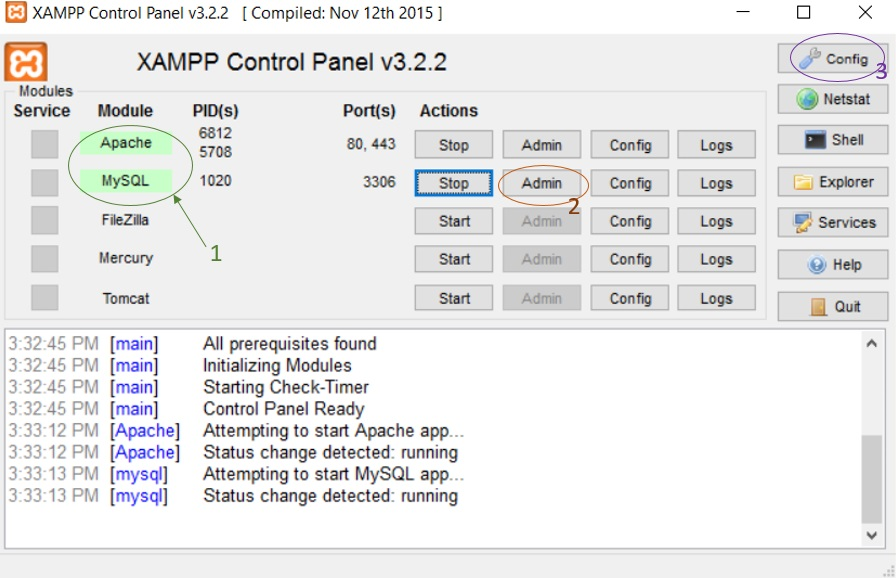
\includegraphics[width=\textwidth]{images/xampp}
    \caption{\footnotesize{1. Shows that both and Apache and MySQL must be 
    running at the same time. 2. The Admin button for mySQL opens phpAdmin 
    which is an graphical interface for accessing the databases in an MySQL 
    server. 3. Configuration button $\rightarrow$ services and ports 
    $\rightarrow$ [MySQL] tab, check that the port is identical to the 
    connected established for WorkBench. The standard is port 3306 }}
\end{figure}

Queries can be executed manually using WorkBench, to follow instructions on how 
to set up a connection for WorkBench, please refer to appendix 
\ref{appen:WorkBench}. Once Work Bench is running properly, it will very 
similar to screen shot provided.
\begin{figure}[!h]
    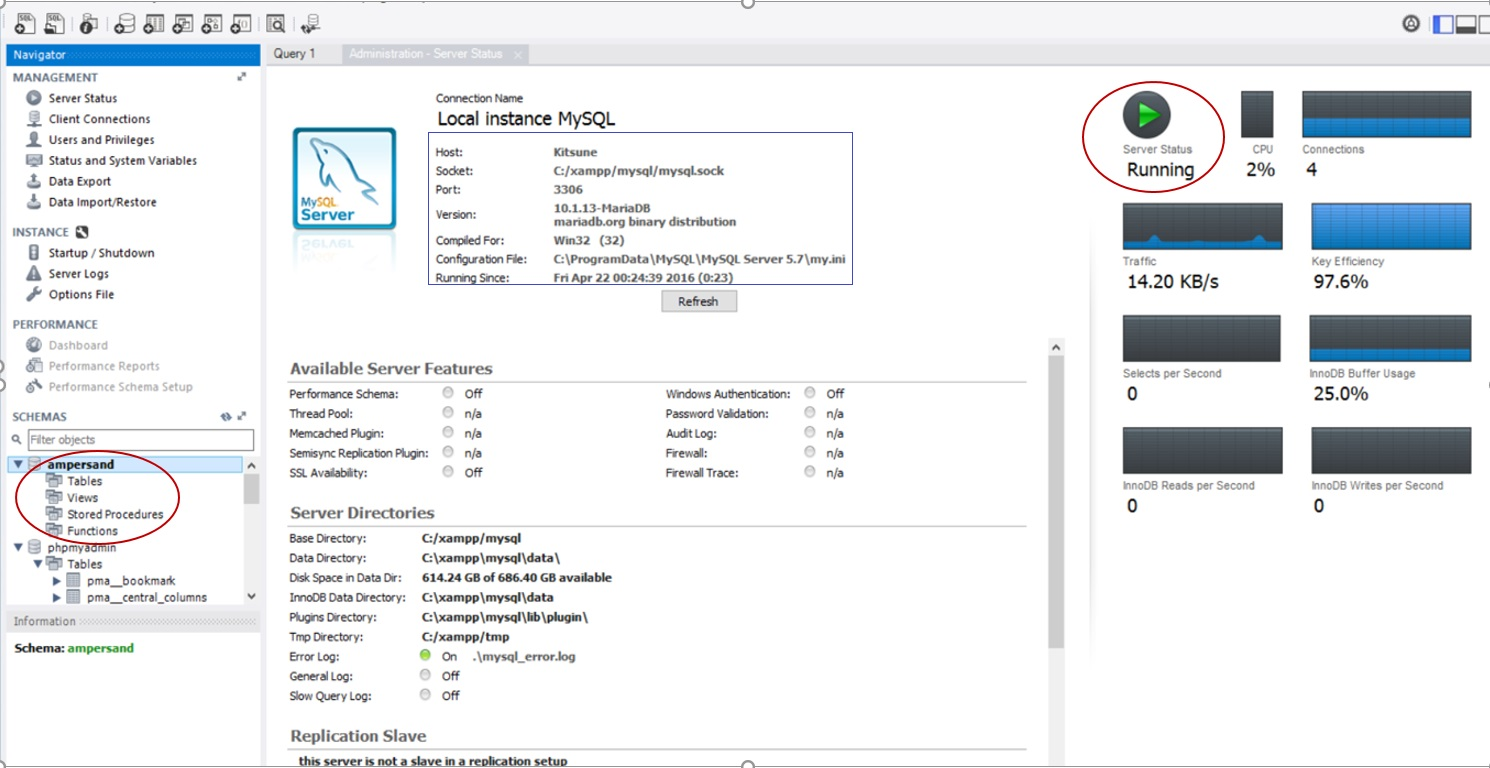
\includegraphics[width=\textwidth]{images/WorkBench}
    \caption{\footnotesize{The right-hand side shows the status of the server, 
    and on the lower left-hand side under 'SCHEMAS', all the databases in 
    current server is listed. Ampersand requires a local database and a 
    password, both of which are 'ampersand'. The blue box in the top middle 
    area provides information concerning the host. }}
\end{figure}

Queries are executed by going to [File] $\rightarrow$ [New Query Tab], a new 
tab will open and one can manually type queries. The execution of these queries 
can be specified to the highlighted portion or everything. The pretty-printer 
outputs onto the command console what is given as output to the Ampersand its 
database. 

\begin{figure}[!h]
    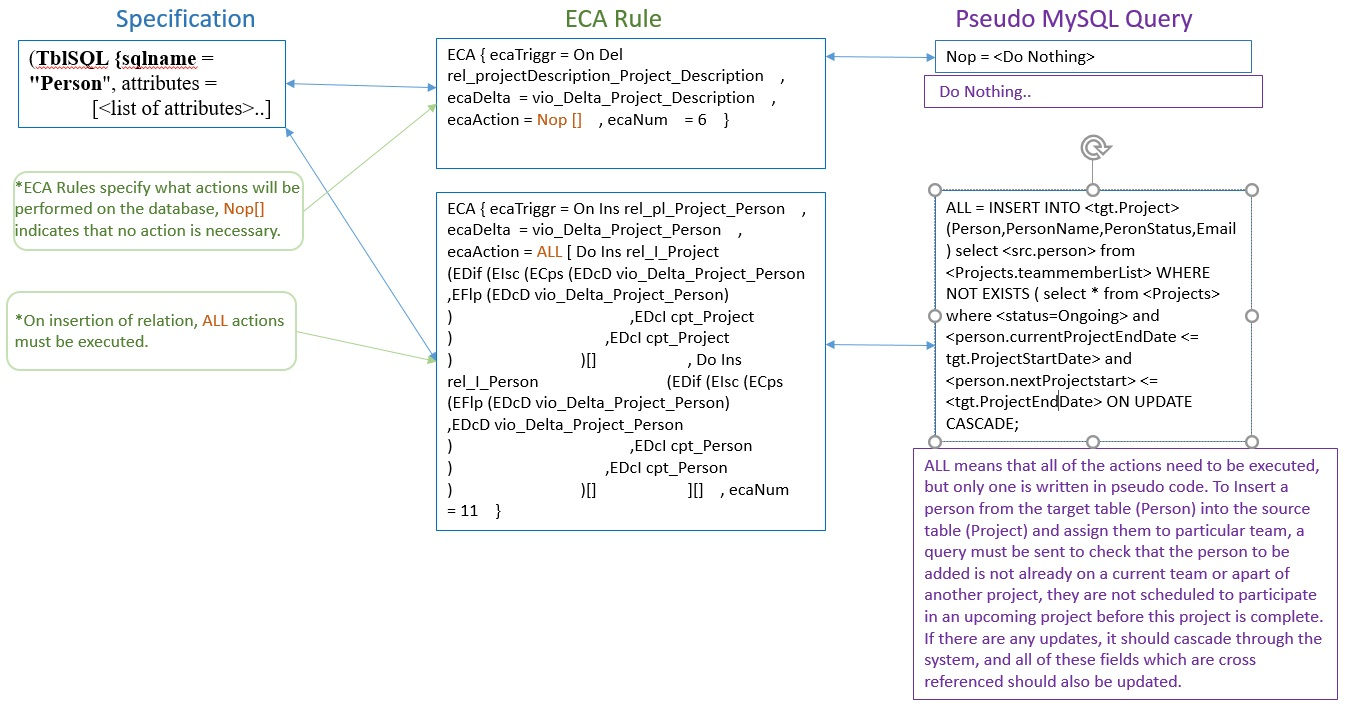
\includegraphics[width=\textwidth]{images/sqlquery}
    \caption{\footnotesize{This figure shows what the system sees in terms of 
    specification, how ECA are structured, and how they are to be executed in 
    SQL. }}
\end{figure}





